\parindent=1cm %красная строка

\begin{center}
		
		\section{Алгоритм роя частиц  переменной окрестности  с отрицательным отбором и его применение}
		
\end{center}

\subsection{Общая идея алгоритма}

Метод роя частиц (МРЧ) использует множество частиц \cite{Eberhart:1995}, \cite{Kondratiev:2010}, каждая из которых представляет потенциальное решение и для каждой частицы можно посчитать фитнес-функцию, служащую для отбраковки худших решений. Изначально множество частиц инициализируется случайными значениями, однако важно, что каждая частица, являющая вектором, должна иметь многомерное равномерное распределение внутри своих значений. Текущая позиция частицы записывается $n$-мерным вектором и обозначается как $X=(X_1,...,X_n)$. i-ый элемент  частицы  в поисковом пространстве S обозначается как $X_i=$ $\begin{bmatrix}
	x_{i1} \\
	
	\vdots \\
	
	x_{iD}
\end{bmatrix}$; текущая скорость частицы обозначается как $V_i=$ 
$\begin{bmatrix}
V_{i1} \\ 

\vdots \\

V_{iD}
\end{bmatrix}$ ; локальная лучшая позиция $P_i$ = $\begin{bmatrix}
P_{i1} 	\\ 

\vdots	\\

P_{iD}
\end{bmatrix}$; глобальное наилучшее решение обозначается как $P_g$ = $\begin{bmatrix}
P_{g1} \\
\vdots \\
P_{gD}	
\end{bmatrix}$. 

Обозначим через $w$ инерционный вес, позволяющий балансировку локального и глобального поиска; $k$ -- номер итерации; $V_{id}$ --скорость частицы $i$ в  $d$-ом пространстве; $r_1, r_2$ -- случайные вещественные числа, такие, что $0 \le r_i \le 1, r_i \in \mathbb{R}, i \in \{1,2\}$; $c_1, c_2$ -- неотрицательные константы, "факторы ускорения".   Скорость и позиция каждой частицы обновляются итеративно по следующей формуле \cite[с. 519]{Cheng:2017}: 
\begin{equation} \label{basic_velocity_and_postion_eq}
	V_{id}^{k} = wV_{id}^{k-1}+c_1r_1(P_{id}^{k-1}-X_{id}^{k-1}) + c_2 r_2(P_{gd}^{k-1} - X_{id}^{k-1}); \\
	X_{id}^{k} = X_{id}^{k-1} + V_{id}^{k}
\end{equation}
 . Для исключения невалидных решений, позиции и скорости частиц ограничены интервалами $[-X_{max}; X_{max}]$ и $[-V_{max}; V_{max}]$ соответственно.

Фитнес каждой частицы вычисляется на каждой итерации; новое значение фитнес-функции сравнивается с текущими локальной и глобальной лучшей позицией; если новое значение превосходит старое, то локальная лучшая позиция будет обновлена и затем среди локальных лучших позиций проводится поиск по максимум фитнес функции; если этот максимум превосходит фитнес функцию глобального лучшего решения, то глобальное лучшее решение заменяется локальным лучшим решением с указанным максимумом. Во избежание зацикливания алгоритма вводится произвольное достаточно большое число $T_{max}$, ограничивающее число итераций алгоритма; в рамках реализации данного алгоритма $T_{max}$ постепенно убывает, что отражает ограниченное время на принятие решения при все более близкой ракете-цели. В конце выполнения алгоритма, наступит ли он сам по достижению заданной точности ли будет прерван $T_{max}$, вектор $P_g$ содержит лучшее решение и представляет собой <<выходные данные>> данного алгоритма.


Общие идеи применения указанного выше алгоритма в этой работе похожи на таковые в работе Ченга, Ли и Зенга \cite{Cheng:2017} и изложены далее. Во-первых, необходимо убедиться в  назначении адекватного кол-ва перехватчиков на одну цель. Для этого сгенерированная и/или обновленная частица должна обновляться по правилу замены повторяющихся элементов в этой частице. Также необходимо избежать выхода скорости частицы за границу $V_{max}$. Для выполнения двух предыдущих условий можно представить формулу \ref{basic_velocity_and_postion_eq} в виде \cite[с. 519]{Cheng:2017}

\begin{equation} \label{advanced_velocity_and_postion_eq}
V^{k} = 
	\begin{cases}
		V_{max}, V^{k} > V_{max} \\
		V^{k}, V_{min} \le V^{k} \le V_{max} \\
		V_{min}, V^{k} < V_{min}
	\end{cases};
X^{k} = 
	\begin{cases}
		X_{max}, X^{k} > X_{max} \\
		X^{k}, X_{min} \le X^{k} \le X_{max} \\
		X_{min}, X^{k} < X_{min}
	\end{cases}
\end{equation}.  \\
В-третьих, для обеспечения более  равномерной сходимости, параметр $w$ будет убывать линейно по формуле \cite[с. 519]{Cheng:2017}: $w = w_{end} + (\frac{T_{max}-k}{T_{max}})(w_0-w{end})$. \\
В-четвертых, $c_1, c_2$ можно использовать не как константы, а переменные, обозначающие фактор самообучения и группового  обучения соответственно и изменяющиеся согласно формуле \cite[с. 519]{Cheng:2017}: 

\begin{equation}
	\begin{cases}
		c_1 = c_{1_{min}} + \frac{(c_{1_{max}} - c_{1_{min}}) k }{T_{max}} \\ 
		c_2 = c_{2_{min}} + \frac{(c_{2_{max}} - c_{2_{min}}) k }{T_{max}}
	\end{cases}
\end{equation}



Введем вспомогательную переменную $K$ -- фактор сужения, необходимый для улучшения сходимости алгоритма. Введем для этого дополнительную переменную $\phi = c_1 + c_2: \phi \ge 2$ и дополнительные обозначения: $N_r$ -- радиус окрестности, меняющийся в ходе итераций; $P_{id}^{k}$ -- собственное экстремальное значение частицы; $P_{N_{r}d}^{k}$ -- экстремальное значение соседа.  Тогда $K = \frac{2}{ \lvert 2 - \phi - \sqrt{\phi ^ 2 - 4 \phi} \rvert}$. С учётом этих нововведений  в практической реализации работы будет использована следующая формула для обновления скорости частицы \cite[с. 520]{Cheng:2017}:

\begin{equation}	\label{best_velocity_and_postion_eq}
	V_{id}^{k} = w V_{id}^{k} - c_1 r_1 (X_{id}^{k-1} - P_{id}^{k-1}) - c_2 r_2 (X_{id}^{k-1} - P_{N_{r}d}^{k-1})
\end{equation}.


Теперь опишем упомянутый в начале главы процесс <<отрицательный отбор>>. <<Отрицательный отбор>> позволяет оптимизировать процесс варьирования окрестности, необходимый чтобы избежать попадания алгоритма в локальный экстремум посредством  обновления некоторых частиц до тех пор, пока не достигнуто условие. Основная идея процесса заключается в итеративном обновлении частиц в соразмерно параметру $R_u$ при сходимости алгоритма. В свою очередь, сходимость алгоритма в процессе его выполнения определяется фактом того, что сходство частиц больше некоторого предела сходства $T_{aff}$. Обозначим сходство частицы $p$ в $d$-ом измерении как $A_{pd}$, $P_{gd}$ -- глобальное экстремальное значение.  %TODO: добавит определение для x 
Сходство частицы $p$ в $d$-ом измерении описывается $A{pd} = 1 + \frac{|P_{gd} - x_{pd}|}{X_{min} - X_{max}}$ \cite[с. 520]{Cheng:2017}.

Также введем формулу для сходства $p$-ой частицы как среднее сходство всех размерностей: $A_{pd} =  \frac {\sum_{d=1}^{D} A_{pd}} {D}$ \cite[с. 520]{Cheng:2017}.

Теперь опишем с помощью простой блок-схемы ниже алгоритм отрицательного отбора для каждой частицы. Заметим, что согласно этой блок-схеме, механизм отрицательного отбора будет задействован только при достижении частицей состояния, в котором  каждая  размерность частицы меньше $T_{aff}$.


\begin{figure*}[h!]
	\centering{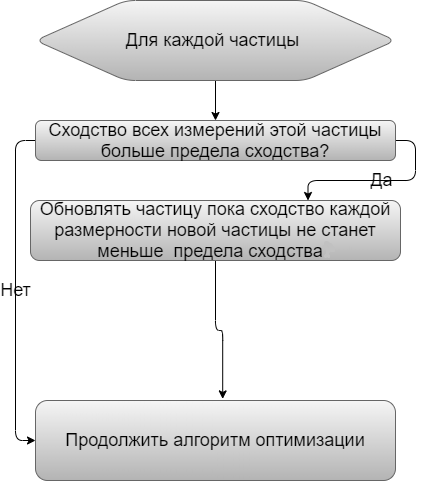
\includegraphics[scale=0.8]{NegativeSelectionProcess.png}}
	\caption{Блок-схема процесса <<отрицательного отбора>>}.
\end{figure*} 

После введения всех необходимых формул, изложения концепций и алгоритмов, играющих вспомогательную роль, опишем непосредственный алгоритм АРЯПОСОО. 

\begin{figure*}
	\centering{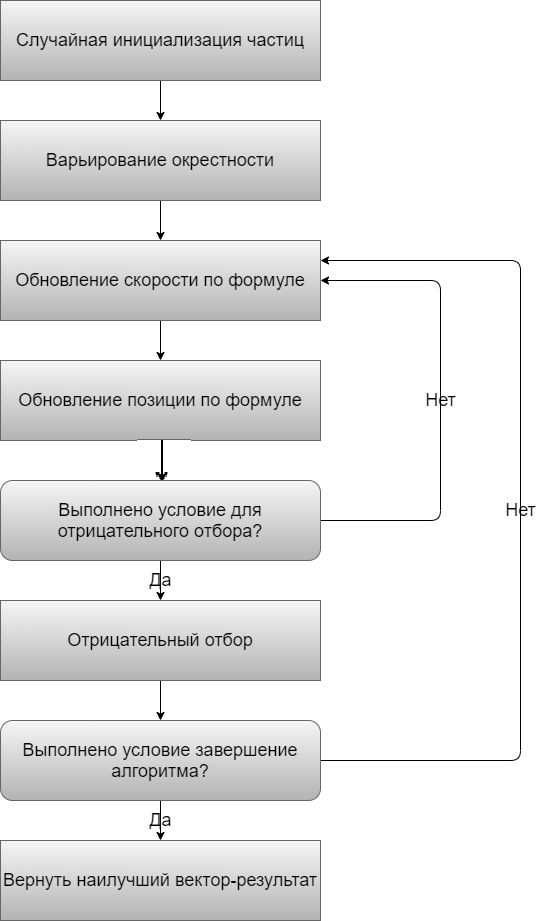
\includegraphics[scale=0.65]{MainAlgorithm.png}}
	\caption{Блок-схема процесса работы алгоритма роя частиц перемененной окрестности с отрицательным отбором}.
\end{figure*} 

\newpage 

\subsection{Реализация алгоритма и интеграция его в СПРО}.

Для быстроты написания, переносимости и использования готовых вспомогательных решений был выбран язык программирования Python 3.7.7. 

Для агентов был введен абстрактный базовый класс <<Abstract Base Class Agent>> и  все используемые агенты являются экземплярами классов-наследников. Компоненты СПРО коммуницируют между собой с помощью веб-сокетов \cite{websockets:git}. Для симуляции передвижения ракет в трехмерном пространстве ракеты хранят на каждой итерации тройку координат внутри своего экземпляра, а <<сканирование>> радаром ракет происходит как анализ всех существующих в данный момент ракет с проверкой нахождения координат внутри области анализа. Возможно, такой подход не является полностью точным, но значительно экономит память и упрощает описание процесса <<сканирования>>; альтернативой данному подходу является создание трехмерного массива, дискретно описывающего пространство. 


Большой трудностью является реализация  одновременно происходящих параллельных событий. Обычно, в студенческих работах  для этого вводят некоторый порядок синхронных непараллельных действий и при этом предполагается, что вычисление этих действий происходит настолько быстро, что время исполнения кода ЦПУ не будет заметным. Однако, алгоритм АРЯПОСОО является затратным по времени, поэтому такой подход в данной работе невозможен.Вместо этого было решено использовать реальное параллельное выполнение кода. Проблемой Python в этой области явлвяется GIL ("Global Interpreter Lock"), однако, этого удалось избежать с использованием Thread- и ProcessPoolExecutor  и запуском каждой ракеты как отдельного процесса  Process.spawn() из модуля multiprocessing. Для реализации одновременности и параллельности каждый компонент выполняется в бесконечном цикле и <<спит>> 0.1 секунды после каждого своего <<тика>> (минимальная единица времени и действия); <<сон>>  с использованием time.sleep() необходим для создания пауз в выполнении кода процессором и переключении контекста выполнения, иначе  потребление ресурсов ЦПУ данным компонентом будет постоянным и вызовет задержки в переключении потока управления, когда число компонентов превысит число логических потоков ЦПУ, что в свою очередь создаст проблемы с симуляцией одновременности. Также заметим, что для быстрого освобождения ресурсов, поток и процесс ракеты при взрыве сразу останавливается и объект ракеты удаляется вручную.

Сама СПРО состоит из генератора атакующих ракет, который с заданной интенсивностью генерирует случайное нормально распределенное на заданному интервале кол-во атакующих ракет с разными параметрами полезной нагрузки, скорости и высоты (для простоты, этот компонент сразу генерирует ракеты находящиеся на этапе прохождения тропосферы), аналогичного генератора ракет-перехватчиков, имитирующего <<подвоз>>  ракет-перехватчиков в случайное время с интенсивностью, возрастающей по мере исчерпания запаса, трех радаров раннего обнаружения, 9 радаров отслеживания и переменного кол-ва ракет-перехватчиков, ограниченных сверху максимальной вместительностью склада, множества защищаемых объектов (программа завершает работу при полном уничтожении всех защищаемых объектов).

Для б$\acute{o}$льшей реалистичности, радары раннего обнаружения, как и радары отслеживания, имеют различный эффективный радиус обнаружения. Для простоты предполагается, что атакующие ракеты входят в имитируемую область <<слева направо>> и все радары <<сканируют область>>, радиус-вектор которой направлен <<слева-направо>>.

Основное принятие решения и генерация плана-перехвата генерируется внутри командного центра, т.е. именно в нём выполняется АРЯПОСОО каждый раз по мере появления новых ракет-целей и ракет-перехватчиков, т.е. при появлении новой ракеты-перехватчика с характеристиками, превосходящими характеристики уже отправленной/отправленных ракеты/ракет и при отсутствии более важных целей, возможно назначение дополнительных ракет. Таким образом, генерация новых планов-перехватов происходит только после наступления события <<новая ракета-цель обнаружена радаром>> или <<на склад поступила новая ракета-перехватчик>>. Также, для реализации неблокирующей работы командного центра (т.е. работы, неблокирующей прием-передачу сигналов), для генерации каждого плана-перехвата создается отдельный процесс с помощью модулю multiporcessing в режиме <<spawn>>, где на каждой итерации проверка каждой частицы на достижение предела сходства происходит внутри отдельного потока внутри ProcessPoolExecutor. Данный подход позволяет максимально задействовать ресурсу ЦПУ при вычислениях  в АРЯПОСОО. 


\subsection{Тестирование и сравнение результатов работы с аналогичными моделями }

Для запуска данной модели был использован компьютер со следующими характеристиками:
OS: Ubuntu 18.04.4 LTS \\
Разрядность: x64 \\
CPU:  Intel(R) Xeon(R) CPU E5-1650 v3 @ 3.50GHz \\
Оперативная память: 126 Гб \\

Самыми важными параметрами является предел сходства $T_aff$ и параметр $R_u$. Для определения оптимального значения этих параметров был проведен оптимизационный эксперимент, результаты которого показаны ниже.


\begin{figure*}[h!]
	\centering{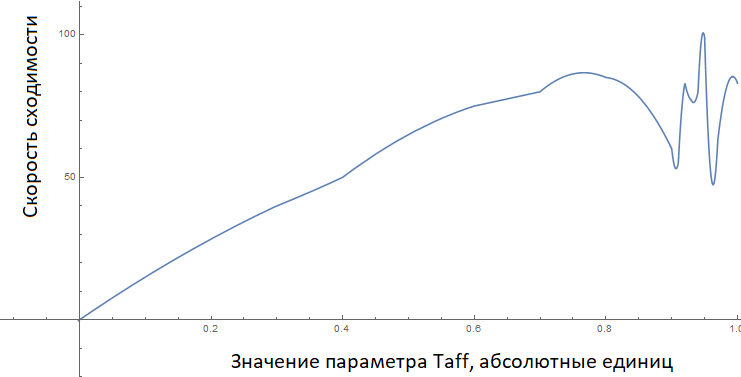
\includegraphics[scale=0.65]{T_aff_ConvergRate.png}}
	\caption{Скорость сходимости алгоритма при различных значениях параметра $T_{aff}$}.
\end{figure*} 

\begin{figure*}[h!]
	\centering{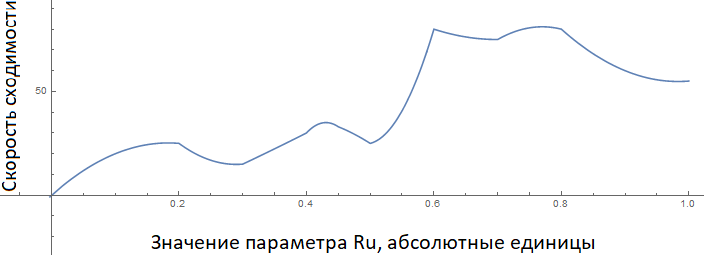
\includegraphics[scale=0.65]{R_u_ConvergRate.png}}
	\caption{Скорость сходимости алгоритма при различных значениях параметра $R_{u}$}.
\end{figure*} 

\newpage

Таким образом, оптимальная скорость сходимости (в процентах от $10^5$ итераций) достигается  в $T_{aff} = 0.96, R_{u} = 0.63$.

Будем считать, что алгоритм сходится  при точности в 99.5$\%$ от оптимального решения. Выполнив $10^6$ итераций каждого алгоритма ниже, имеем следующие скорости сходимости и среднее кол-во итераций, \cite[с. 521]{Cheng:2017}.


\begin{table}[]
	\begin{tabular}{lll}
		Алгоритм  & Средняя скорость сходимости, \% & Среднее кол-во итераций \\
		PSO       & 80.3                    & 975                     \\
		CFPSO     & 85.1                    & 937                     \\
		LDPSO     & 87.6                    & 850                     \\
		VNPSO     & 91.5                    & 715                     \\
		VNVNNSPSO & 96.8                    & 720                     \\
		АРЯПОСОО  & 92.333                  & 698                    
	\end{tabular}
	\caption{Скорость сходимости и среднее кол-во итераций различных методов}
	\label{tab:converg_rate_and_avg_iters_number}
\end{table}

Как видим, несмотря на не самый лучший результат в средней скорости сходимости, алгоритм АРЯПОСОО работает быстрее всех остальных, что позволяет использовать его как основной, если задача, к которой он применяется, ограничена по времени \cite[с. 522-524]{Cheng:2017}. 

Разработанная  программа генерирует планы-перехваты подобного вида:



\begin{figure*}[]
	\centering{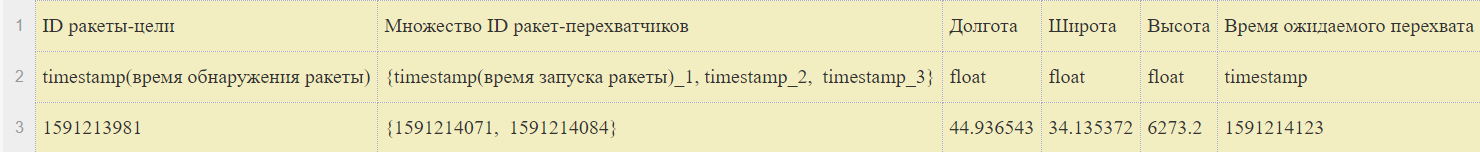
\includegraphics[scale=0.5]{CapturePlanExample.png}}
	\caption{Пример плана-перехвата, генерируемого программой (пост-визуализация в стороннем ПО)}.
\end{figure*} 

\newpage

Выходной формат .csv позволяет импортировать данные в любой табличный процессор для последующей их обработки и визуализации. Во избежание ситуации неправильного вывода, формируемого при многопоточной работе приложения, вывод данных на консоль или файл осуществляет отдельный поток.
